\documentclass[a4paper,12pt]{article}

\usepackage[a4paper,left=2.54cm,right=2.54cm,top=2.54cm,bottom=2.54cm]{geometry}

\usepackage[croatian]{babel}
\usepackage[utf8]{inputenc}
\usepackage{times}

\usepackage{amsmath} 
\usepackage{amssymb}

\usepackage{setspace}
\onehalfspacing

\usepackage{titlesec}
\titleformat{\section}{\fontsize{16pt}{20pt}\selectfont\bfseries}{\thesection.}{0.4cm}{}
\titleformat{\subsection}{\fontsize{14pt}{18pt}\selectfont\bfseries}{\thesubsection.}{0.4cm}{}
\setlength{\parskip}{10pt}

\titlespacing*{\section}{0pt}{0.5cm}{0pt}
\titlespacing*{\subsection}{0pt}{0.5cm}{0pt}

\usepackage{enumitem}
\setlist{topsep=3pt,itemsep=3pt}

\usepackage{graphicx,caption}

\usepackage[numbers]{natbib}
\setlength{\bibsep}{2pt}
\newcommand\tab[1][1cm]{\hspace*{#1}}


\begin{document}

%%%%%%%%%%%%%%%%%%%%%%%%%%% NASLOVNICA %%%%%%%%%%%%%%%%%%%%%%%%%%%%%%%%%%%%%%%%%%%%%%%%%%%
\thispagestyle{empty}
\begin{center}
Sveučilište u Zagrebu\\
Fakultet organizacije i informatike
\end{center}
\vfill
\begin{center}
\Large Uvod u THREEjs
\end{center}
\vfill
\begin{flushright}
Tim: Karlo Jačmenjak \break
Antonio Kupčić \break
Josip Mojzeš \break
\end{flushright}
U Varaždinu, 2.1.2023. 

\newpage
\setcounter{page}{1}
%%%%%%%%%%%%%%%%%%%%%% KRAJ NASLOVNICE %%%%%%%%%%%%%%%%%%%%%%%%%%%%%%%%%%%%%%%%%%%%%%%%%%%

\section{Uvod}

\textbf{THREE.js} je JavaScript cross platform biblioteka i sučelje za programiranje aplikacija (API) koje se koristi za stvaranje i prikaz animirane 3D računalne grafike u web pregledniku pomoću WebGL-a. Izvorni kod THREE.js-a je otvorenog tipa.

\section{Zadatak 1.}
\subsection{Postavljanje kamere}
\begin{flushleft}
    Za početak rada u THREE.js prvo moramo dobiti WebGL kontekst i stvoriti novu scenu 
\end{flushleft}


\begin{figure}[ht]
    \centering
    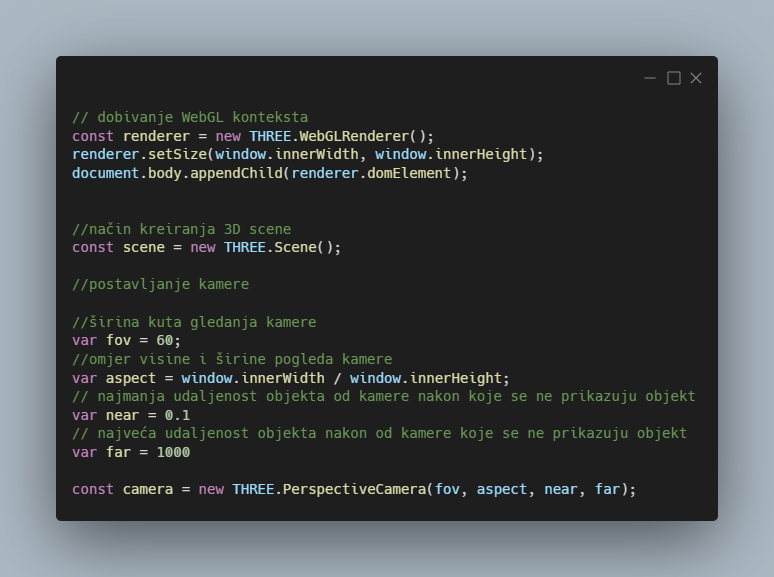
\includegraphics[scale=0.5]{image/zadatak1.png}
    \caption{Primjer koda za postavljanje kamere.}
\end{figure}


Dakle kao što vidimo na slici 3D scena se kreira na Three.Scene() funkcijom. Da bi smo postavili kameru trebamo koristiti četiri varijable, a to su 
varijabla \textit{fov} koja se koristi za širinu kuta gledanja, \textit{aspect} za omjer visine i širine pogleda pomoću ugrađenih objekata browsera, \textit{near} je 
varijabla koja se koristi za predstavljanje najmanje udaljenosti gdje se objekt ne prikazuje na kameri te varijabla \textit{far} koja je predstavljanje najveću 
udaljenost gdje se objekt ne prikazuje na kameri.
varijabla \textit{camera} služi tome da se prije navedene četiri varijable stave kao parametri u funkciju \texttt{PerspectiveCamera}.
\subsection{Kreiranje scene i objekta}
\begin{figure}[ht]
    \centering
    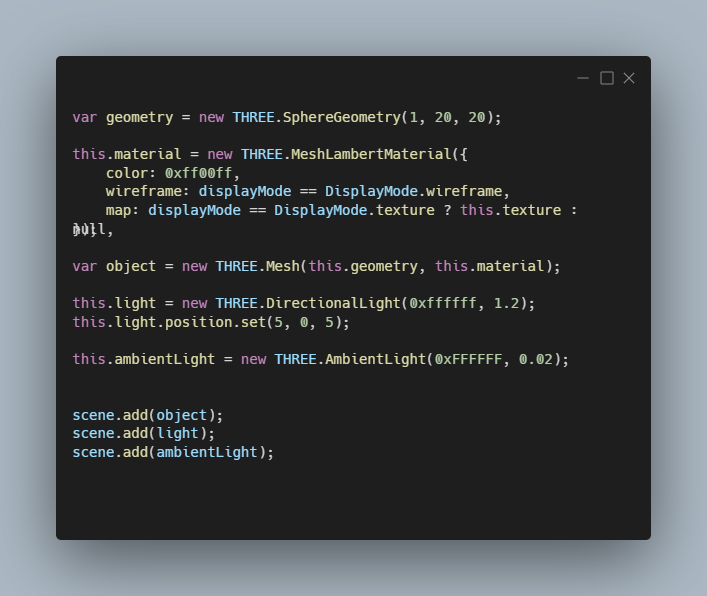
\includegraphics[scale=0.5]{image/zadatak1_objekti.png}
    \caption{Primjer koda za dodavanje objekta sceni te postavljanje svijetlosti i materijala.}
\end{figure}


Da bi smo dodali objekt u scenu moramo napraviti varijablu \textit{object} koja je predstavlja fukciju \texttt{Mesh}. \texttt{Mesh} je funkcija koja poprima dva parametra, a to su materijal i 
vrstu geometrijskog tijela. U kodu na slici se radi o sferi pa se prvo mora stvoriti varijabla \textit{geometry} koja predstavlja funkciju \texttt{SphereGeometry} koja stvara sferu.
Drugi parametar funkcije \texttt{Mesh} je material. \textit{Material} je također varijabla koja predstavlja funkciju \texttt{MeshLamberMaterial} koja stvara materijal prema određenoj boji, 
prikazu i teksturi. Kada smo to sve napravili tada možemo pozvati \texttt{add} funkciju da stvorimo objekt. Svijetlo  se također postavlja sa \texttt{add}.
Varijabla \textit{light} predstavlja funkciju \texttt{DirectionalLight} koja stvara svijetlost te tu svijetlost postavljamo na neku poziciju. 
\pagebreak
\subsection{Interakcija miša i tastature s scenom.}
\begin{figure}[ht]
    \centering
    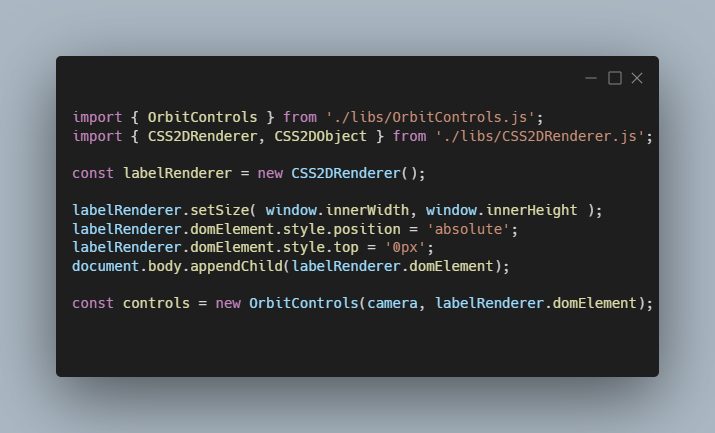
\includegraphics[scale=0.5]{image/zadatak1_kontrole.png}
    \caption{Primjer koda za interakciju miša i tastature s scenom.}
\end{figure}

Interakcija preko miša i tastature se implementira se postiže sa objektima OrbitControls i renderer. Orbit controls omogućava da se kamera kreće oko modela,
a CSS2DRenderer prikazuje sve potrebne elemente modela.

\pagebreak
\section{Zadatak 2.}

\subsection{Matematički model mrežastog prikaza za valjak}
\begin{center}
    \begin{tabular}{||c | c | c | c ||} 
     \hline
     vrh & x & y & z \\ [0.5ex] 
     \hline
     $A_1$ & 1 & 1 & 0  \\ 
     \hline
     $A_2$ & $\sqrt{2}$ & 0 & 0  \\
     \hline
     $A_3$ & 1 & -1 & 0  \\
     \hline
     $A_4$ & 0 & -$\sqrt{2}$ & 0 \\
     \hline
     $A_5$ & -1 & -1 & 0  \\ 
     \hline
     $A_6$ & -$\sqrt{2}$ & 0 & 0  \\
     \hline
     $A_7$ & -1 & 1 & 0  \\
     \hline
     $A_8$ & 0  & $\sqrt{2}$ & 0 \\
     \hline
     $A_9$ & 1 & 1 & 2  \\
     \hline
     $A_{10}$& $\sqrt{2}$ & 0 & 2 \\
     \hline
     $A_{11}$ & 1 & -1 & 2  \\
     \hline
     $A_{12}$ & 0 & $\sqrt{2}$ & 2 \\
     \hline
     $A_{13}$ & -1 & 1 & 2  \\ 
     \hline
     $A_{14}$ & -$\sqrt{2}$ & 0 & 2  \\
     \hline
     $A_{15}$ & -1 & -1 & 2  \\
     \hline
     $A_{16}$ & 0 & -$\sqrt{2}$ & 2  \\
     \hline
     $A_{17}$ & 0  & 0 & 0 \\
     \hline
     $A_{18}$ & 0 & 0  & 2\\ [1ex] 
     \hline
    \end{tabular}
    \end{center}

    \begin{figure}[ht]
        \centering
        \caption{Tablica točaka.}
    \end{figure}

    \begin{center}
        \begin{tabular}{||c | c | c ||} 
         \hline
         edge & početak & kraj  \\ [0.5ex] 
         \hline
         $e_1$ & $A_{1}$ & $A_{2}$ \\ 
         \hline
         $e_2$ & $A_{2}$ & $A_{3}$  \\
         \hline
         $e_3$ & $A_{3}$ & $A_{4}$  \\
         \hline
         $e_4$ & $A_{4}$ & $A_{5}$  \\
         \hline
         $e_5$ & $A_{5}$ & $A_{6}$ \\ 
         \hline
         $e_6$ & $A_{6}$ & $A_{7}$  \\
         \hline
         $e_7$ & $A_{7}$ & $A_{8}$  \\
         \hline
         $e_8$ & $A_{8}$  & $A_{1}$ \\
         \hline
         $e_9$ & $A_{9}$ & $A_{10}$  \\
         \hline
         $e_{10}$& $A_{11}$ & $A_{16}$ \\
         \hline
         $e_{11}$ & $A_{16}$ & $A_{15}$   \\
         \hline
         $e_{12}$ & $A_{15}$ & $A_{14}$  \\
         \hline
         $e_{13}$ & $A_{13}$ & $A_{12}$   \\ 
         \hline
         $e_{14}$ & $A_{12}$ & $A_{9}$  \\
         \hline
         $e_{15}$ & $A_{9}$ & $A_{9}$  \\
         \hline
         $e_{16}$ & $A_{10}$ & $A_{2}$  \\
         \hline
         $e_{17}$ & $A_{11}$  & $A_{3}$ \\
         \hline
         $e_{18}$ & $A_{16}$ & $A_{4}$ \\ 
         \hline
         $e_{19}$& $A_{15}$ & $A_{5}$ \\
         \hline
         $e_{20}$ & $A_{14}$ & $A_{6}$   \\
         \hline
         $e_{21}$ & $A_{13}$ & $A_{7}$  \\
         \hline
         $e_{22}$ & $A_{12 }$& $A_{8}$ \\ 
         \hline
         $e_{23}$ & $A_{1}$ & $A_{17}$  \\
         \hline
         $e_{24}$ & $A_{1}$ & $A_{17}$   \\
         \hline
         $e_{25}$ & $A_{2}$ & $A_{17}$   \\
         \hline
         $e_{26}$ & $A_{3}$  & $A_{17}$  \\
         \hline
         $e_{27}$ & $A_{4}$ & $A_{17}$  \\ 
         \hline
         $e_{28}$& $A_{5}$ & $A_{17}$  \\
         \hline
         $e_{29}$ & $A_{6}$ & $A_{17}$  \\
         \hline
         $e_{30}$ & $A_{7}$0 & $A_{17}$  \\
         \hline
         $e_{31}$ & $A_{8}$ & $A_{17}$  \\ 
         \hline
         $e_{32}$ & $A_{9}$ & $A_{18}$  \\
         \hline
         $e_{33}$ & $A_{10}$ & $A_{18}$   \\
         \hline
         $e_{34}$ & $A_{11}$ & $A_{18}$   \\
         \hline
         $e_{35}$ & $A_{12}$  &$A_{18}$  \\
         \hline
         $e_{36}$ & $A_{13}$ &$A_{18}$  \\ 
         \hline
         $e_{37}$& $A_{14}$ & $A_{18}$  \\
         \hline
         $e_{38}$ & $A_{15}$ & $A_{18}$   \\
         \hline
         $e_{39}$ & $A_{16}$ &$A_{18}$ \\[1ex] 
         
        \end{tabular}
        \end{center}
        \begin{figure}[ht]
            \centering
            \caption{Tablica rubova.}
        \end{figure}

    \subsection{Matematički model mrežastog prikaza za stošca}
\begin{flushleft}
    \begin{tabular}{||c | c | c ||} 
     \hline
     edge & start & end \\ [0.5ex] 
     \hline\hline
     1 & 6 & 87837  \\ 
     \hline
     2 & 7 & 78  \\
     \hline
     3 & 545 & 778  \\
     \hline
     4 & 545 & 18744 \\
     \hline
     5 & 88 & 788  \\ [1ex] 
     \hline
    \end{tabular}
    \end{flushleft}

    \subsection{Matematički model mrežastog prikaza za sfere}
\begin{flushleft}
    \begin{tabular}{||c | c | c ||} 
     \hline
     edge & start & end \\ [0.5ex] 
     \hline\hline
     1 & 6 & 87837  \\ 
     \hline
     2 & 7 & 78  \\
     \hline
     3 & 545 & 778  \\
     \hline
     4 & 545 & 18744 \\
     \hline
     5 & 88 & 788  \\ [1ex] 
     \hline
    \end{tabular}
    \end{flushleft}

\newpage
\subsection{Phongov model osvjetljenja}
Phongov model osvjetljenja je računalni model koji se koristi u računalnoj grafici za simuliranje osvjetljenja na površinama objekata u 3D prostoru. Model se zasniva na matematičkom modelu osvjetljenja koji je razvio Bui Tuong Phong, a koji se temelji na fizičkim zakonima o refleksiji svjetlosti.

Model osvjetljenja Phonga opisuje osvjetljenje površine objekta kao linearnu kombinaciju tri komponente: ambijentalne, difuzne i spekularne refleksije.

Ambijentalna refleksija je svjetlost koja dolazi sa svih smjerova i koja se reflektira jednako u svim smjerovima. Ova komponenta se koristi za simuliranje svjetlosti koja dolazi iz okoliša i koja se odbija sa površine objekta.

Difuzna refleksija je svjetlost koja se odbija od površine objekta u svim smjerovima jednako, bez obzira na smjer iz kojeg dolazi. Ova komponenta se koristi za simuliranje svjetlosti koja se odbija od objekta u zavisnosti od njegove boje i teksture.

Spekularna refleksija je svjetlost koja se odbija od površine objekta u jednom specifičnom smjeru. Ova komponenta se koristi za simuliranje bljeska i odsjaja na površini objekta.

Phongov model osvjetljenja se često koristi u računalnoj grafici jer je jednostavan za implementiranje i daje realistične rezultate u većini slučajeva. Međutim, postoje i druge metode za simuliranje osvjetljenja u računalnoj grafici, kao što su radiosity i ray tracing, koje su možda preciznije ali i skuplje za implementiranje.
\subsection{Gouraud i Phong sjenčanje}

Gouraud sjenčanje (ili glatko sjenčanje) je izračunavanje boja po vrhovima. 
To znači da sjenčilo vrhova mora odrediti boju za svaki vrh i proslijediti boju kao izlaznu varijablu sjenčilu fragmenta. 
Budući da se ova boja prosljeđuje sjenčilu fragmenata kao promjenjiva varijabla, interpolira se preko fragmenata dajući glatko sjenčanje.

Nasuprot tome, Phong sjenčanje je izračunavanje boje po fragmentu. 
Osjenčivač vrhova daje podatke o normalama i podatke o položaju kao izlazne varijable za sjenčilo fragmenta. 
Sjenčalo fragmenta zatim interpolira te varijable i izračunava boju.

\subsection{Neka svojstva materijala}
\subsubsection{MeshBasicMaterial}

\hspace{10mm} Materijal za crtanje geometrija na jednostavno osjenčan (ravan ili žičani) način.

\subsubsection{MeshDepthMaterial}
\hspace{10mm} Materijal za crtanje geometrije po dubini. Dubina se temelji na bliskoj i dalekoj ravnini kamere. Bijelo je najbliže, crno je najdalje.

\subsubsection{MeshDistanceMaterial}
\hspace{10mm} MeshDistanceMaterial interno se koristi za implementaciju mapiranja sjena pomoću PointLighta .

\subsubsection{MeshLambertMaterial}
Materijal za nesjajne površine, bez odsjaja.
Materijal koristi nefizički zasnovan Lambertov model za izračun refleksije. Ovo može dobro simulirati neke površine (kao što je neobrađeno drvo ili kamen), ali ne može simulirati sjajne površine sa reflektirajućim odsjajima (kao što je lakirano drvo). MeshLambertMaterial koristi sjenčanje po fragmentu.

\pagebreak
\subsection{Neka svojstva svjetlosti}
\subsubsection{AmbientLight}
\hspace{10mm} Ovo svjetlo globalno jednako osvjetljava sve objekte u sceni.
Ovo se svjetlo ne može koristiti za bacanje sjena jer nema smjer.

\subsubsection{DirectionalLight}
\hspace{10mm} Svjetlost koja se emitira u određenom smjeru. Ovo svjetlo će se ponašati kao da je beskrajno daleko i da su zrake koje iz njega proizlaze sve paralelne. Uobičajen slučaj za ovo je simulacija dnevnog svjetla; sunce je dovoljno daleko da se njegov položaj može smatrati beskonačnim, a sve svjetlosne zrake koje dolaze s njega su paralelne.

\subsubsection{SpotLight}
\hspace{10mm} Ovo svjetlo se emitira iz jedne točke u jednom smjeru, duž stošca koji se povećava što je dalje od svjetla.

\pagebreak
\subsection{Neka svojstva svjetlosti}
\subsubsection{AmbientLight}
\hspace{10mm} Ovo svjetlo globalno jednako osvjetljava sve objekte u sceni.
Ovo se svjetlo ne može koristiti za bacanje sjena jer nema smjer.

\subsubsection{DirectionalLight}
\hspace{10mm} Svjetlost koja se emitira u određenom smjeru. Ovo svjetlo će se ponašati kao da je beskrajno daleko i da su zrake koje iz njega proizlaze sve paralelne. Uobičajen slučaj za ovo je simulacija dnevnog svjetla; sunce je dovoljno daleko da se njegov položaj može smatrati beskonačnim, a sve svjetlosne zrake koje dolaze s njega su paralelne.

\subsubsection{SpotLight}
\hspace{10mm} Ovo svjetlo se emitira iz jedne točke u jednom smjeru, duž stošca koji se povećava što je dalje od svjetla.

\pagebreak


\section{Zadatak 3.}
Najučinkovitiji način za transformiranje koordinata u trodimenzionalnom prostoru je uporabom
linearnog operatora, odnosno matrica transformacija. U nastavku su prikazane matrice transformacija
za translacija, skaliranje te rotaciju oko x, y i z osi koje Three.js koristi.

Translacija
\[
T_{tx,ty,tz}=
\begin{bmatrix}
    1 & 0 & 0 & tx \\
    0 & 1 & 0 & ty \\
    0 & 0 & 1 & tz \\
    0 & 0 & 0 & 1
\end{bmatrix}
\]

Skaliranje
\[
S_{k}=
\begin{bmatrix}
    k & 0 & 0 & 0 \\
    0 & k & 0 & 0 \\
    0 & 0 & k & 0 \\
    0 & 0 & 0 & 1
\end{bmatrix}
\]

Rotacija oko x osi

\[
R_{x,\theta}=
\begin{bmatrix}
    1 & 0 & 0 & 0 \\
    0 & \cos{\theta} & -\sin{\theta} & 0 \\
    0 & \sin{\theta} & \cos{\theta} & 0 \\
    0 & 0 & 0 & 1
\end{bmatrix}
\]

Rotacija oko y osi
\[
R_{y,\theta}=
\begin{bmatrix}
    \cos{\theta} & 0 & \sin{\theta} & 0 \\
    0 & 1 & 0 & 0 \\
    -\sin{\theta} & 0 & \cos{\theta} & 0 \\
    0 & 0 & 0 & 1
\end{bmatrix}
\]

Rotacija oko z osi
\[
R_{z,\theta}=
\begin{bmatrix}
    \cos{\theta} & -\sin{\theta} & 0 & 0 \\
    \sin{\theta} & \cos{\theta} & 0 & 0 \\
    0 & 0 & 1 & 0 \\
    0 & 0 & 0 & 1
\end{bmatrix}
\]

\pagebreak

Da se neka transformacija $T$ može primijeniti na određene koordinate $(x, y, z)$, koordinate je
potrebno zapisati u matričnom zapisu $M_{x,y,z}$. Zatim se primjenjuje matrično množenje
matrica $M_T$ i $M_{x,y,z}$, gdje je $M_T$ matrica transformacije $T$.

\[
M_{x,y,z}=
\begin{bmatrix}
    x \\
    y \\
    z \\
    1
\end{bmatrix}
\]
\pagebreak

\section{Zadatak 4.}
\pagebreak

\section{Zadatak 5.}
\pagebreak
\section{Zadatak 6.}
\pagebreak
\section{Zadatak 7.}
\begin{figure}[ht]
    \centering
    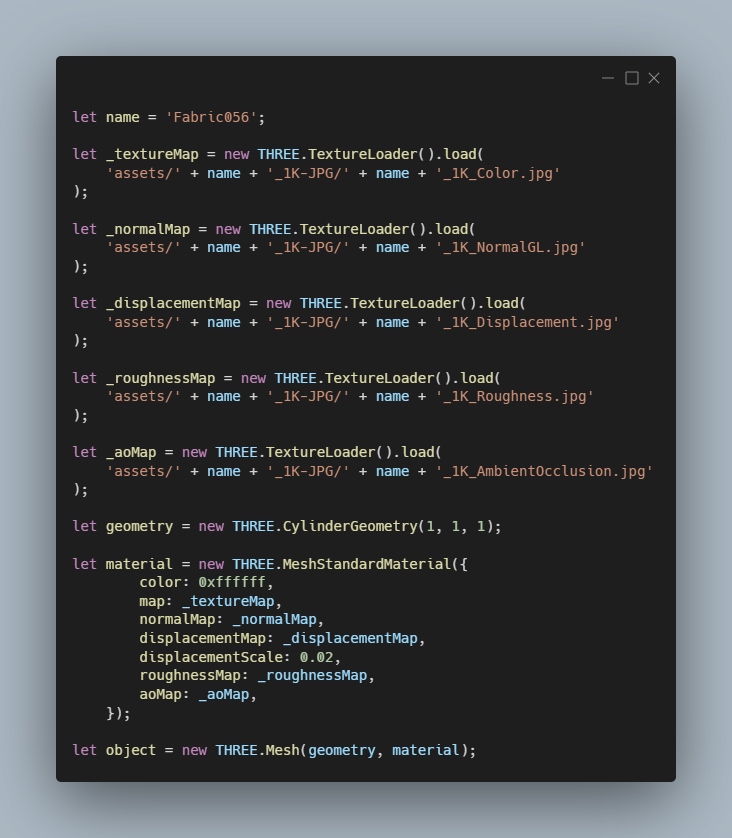
\includegraphics[scale=0.5]{image/zadatak7.png}
    \caption{Inicijaliziranje teksture.}
\end{figure}

\textit{NormalMap} je proces stvaranja detaljne grafike pomoću tekstura koje se "mapiraju" na 3D objekte. Ova tehnika se koristi za stvaranje iluzije neravnina i udubljenja na objektima pomoću tekstura koje imitiraju sjene i promjene boje u različitim uvjetima osvjetljenja.
\newline \textit{DisplacementMap} je tehnika koja se koristi u računalnoj grafici za stvaranje iluzije promjena u položaju točaka na površini objekta. Ova metoda se razlikuje od drugih tehnika poput preslikavanja neravnina, normale i paralakse jer koristi mapu teksture ili visine
umjesto geometrijskih podataka o položaju točaka. Kada se mapiranje pomaka primjenjuje, vrijednosti iz mape teksture se koriste za procjenu pomaka točaka duž normale lokalne površine. Ova tehnika se koristi za stvaranje efekata poput valova ili udubljenja na površini objekta.
\newline \textit{Roughness map} je podatkovna struktura koja se koristi u računalnoj grafici za definiranje kako se svjetlost odbija s površine 3D modela. Vrijednosti u ovoj mapi se koriste za procjenu koliko će površina biti sjajna ili mat. Vrijednosti bliže nuli (0) rezultiraju vrlo sjajnom površinom, 
poput plastike, dok vrijednosti bliže jedinici (1) rezultiraju mat izgledom. Ova karta se koristi za stvaranje realističnih učinaka odbijanja svjetlosti na površini 3D modela
\pagebreak
\section{Zadatak 8.}
\pagebreak

\paragraph{Referenciranje na literaturu.} Prema literaturi \cite{Maric} vrijedi\,\ldots \ Prema literaturi \cite{geo} mora biti\,\ldots

\begin{thebibliography}{9}

\bibitem{Youtube} Jeff Anderson \emph{Applied Linear Algebra, Lesson 7, Video 5: Wireframe Model in 3D} \texttt{https://www.youtube.com/watch?v=FDDl5PQBAkM} (3.1.2023.)
\bibitem{Youtube} Jeff Anderson \emph{Applied Linear Algebra, Lesson 7, Video 6: Wireframe Model in 3D} \texttt{https://www.youtube.com/watch?v=6KJH1dG8qLY} (3.1.2023.)
\bibitem{Youtube} Jeff Anderson \emph{Applied Linear Algebra, Lesson 7, Video 7: Wireframe Model in 3D} \texttt{https://www.youtube.com/watch?v=YaxuxZiXnKI} (3.1.2023.)
\bibitem{three} Three.js, \texttt{https://threejs.org/}, (28.12.2022.)
\bibitem{geo} GeoGebra, \texttt{http://www.geogebra.org/cms/}, (4.1.2023.)
\bibitem{haroldserrano}  13.5.2016. Harold Serrano \emph{What is the difference between Gouraud and Phong shading?} https://www.haroldserrano.com/blog/what-is-the-difference-between-gouraud-and-phong-shading (4.1.2023.)
\bibitem{wiki} \emph{Normal mapping} \texttt{https://en.wikipedia.org/wiki/Normal\_mapping} (5.1.2023.)
\end{thebibliography}

\end{document}